\documentclass{article}

\usepackage[margin=0.8in]{geometry}
\usepackage{subfig}
\usepackage{amsmath}
\usepackage{amsfonts}
\usepackage{amssymb}
\usepackage{amsthm}
\usepackage{graphicx}
\usepackage[hidelinks]{hyperref}
\usepackage{showlabels}
\usepackage{lineno}
% \linenumbers
\usepackage{natbib}

\newtheorem{lemma}{Lemma}
\newtheorem{prop}{Proposition}
\newtheorem{thm}{Theorem}
\newtheorem{prob}{Problem}
\newtheorem{defn}{Definition}
\newtheorem{obs}{Observation}
\newtheorem{alg}{Algorithm}

\newcommand{\median}{\operatorname{median}}

% http://bytesizebio.net/2013/03/11/adding-supplementary-tables-and-figures-in-latex/
\newcommand{\beginsupplement}{%
        \setcounter{table}{0}
        \renewcommand{\thetable}{S\arabic{table}}%
        \setcounter{figure}{0}
        \renewcommand{\thefigure}{S\arabic{figure}}%
     }

\hyphenation{Ge-nome Ge-nomes hyper-mut-ation through-put}

\title{Fall Internship Report: A literature review on quantitative assays immunology}
\author{Jared Galloway}

\begin{document}
\maketitle

\begin{abstract}
Protection from rapidly evolving and spreading viruses is key to human health and survival.
The molecular nature of infection and immune system defences provides us with a complex and noisy set of of problems to solve
if we are to combat infectious disease and understand the nature of their evolution.
Most notably, we need to understand the binding affinity of a virus to bind to a host cell via proteins on the expressed on the surface of the cell's outer membrane.
These proteins allow the virus to enter a host cell, then proceed to hijack the cell's own machinery to replicate and propagate an infection.
In the context of SARS-CoV-2, understanding the immune response with respect to those binding proteins is critical
for prevention and prediction of disease severity.
Additionally, understanding the evolution of these binding sites allows us to interpret the cross-species transmission
and duration of immunity post-infection, or the potential mutational routes of binding escape.
Neither of these are trivial problems to solve. 
Fortunately, recent advances in next generation sequencing (NGS), oligonucleotide synthesis (ONS), and PCR-induced <?>
have driven the development of quantitative assays and given us the ability to explore and quantify fitness of particular sequences in the context of protein interaction.
These methods have laid the foundation for exploration and development of advanced vaccines providing protection against deadly pathogens
from causing serious illness and even death.
In this literature review, we explore the advanced quantitative assays, Phage Immunoprecipitation Sequencing
and Deep Mutational Scanning, which allow us to measure and explore these complex and noisy problems.
Concretely, we will observe the results and methods from \citet{Shrock2020} and \citet{Starr2020}, 
two papers that focus on the binding properties of the novel betacoronavirus, SARS-CoV-2.
% Further we explore the modeling and analysis techniques necessary to parse and query the resulting data from these protocols.
\end{abstract}


\section*{Introduction}

% Introduce the immune system
Modern mammalian immune systems are constituted by the aggregate of proteins and cells which
defend against unwanted invaders (pathogens).
These defences keep the pathogens from harming the delicate and complex biological systems which keep us alive and healthy.
However, deadly pathogenic outbreaks which rapidly spread among humans and other species can often harm or kill a large percentage of populations \citep{Wu2020}.
In the case of viruses, replication as a function of fitness drives pathogens to evolve much in the same way we do --
often meaning the most potent and infectious pathogens prevail as a product of their genome evolution \citep{Twiddy2003, Felsenstein1981-zs}.
Fighting fire with fire, the adaptive immune system works through similar processes of mutation and selection, inside our own body,
to evolve along-side these pathogens and confer specialized immunity - in many cases lasting throughout the lifetime of an individual.
Incredibly, the combinatorial effects of specialized (VDJ) recombination results in enough diversity to select upon that evolution of specialized cells
takes place in mere days (often a week or so) when encountering a new pathogen \citep{Jung2004}.

~
% Motivate the importance of quantitative assays.
In contrast to all other forms of evolution (often on ecological timescales), 
The process of generating specific antibodies to ward off an infection is incredibly fast.
Unfortunately, the symptoms of an infection during that time frame can still make an individual very ill, or even be fatal.
The ability of viruses to hijack our cell's own machinery to replicate itself in order to propagate the infection make them effecient and deadly.
Luckily, the process of producing antibodies need not occur everytime we ecounter the same virus.
Rather, once an individual has encountered a pathogen and created the necessary cells needed to fend off the virus and infected cells,
the defences that were used are stored in a sort of ``immuno-memory" -- using another type specialized cell.
Upon contact with a pathogen the individual has encountered in the past, then,
the immune system has the infrastructure in place to elicit a fast and effective response, 
Having this cellular machinery is what's known as immunity in an individual - and is key to survival in a world filled with microbial pathogens.
One of the most impactful developments in human health has been our ability to provoke immunity to common
viruses without actually infecting us with a deadly disease causing pathogen.
These biologically prepared agents are known as \textit{vaccines}, 
and according to the center for disease control (CDC.gov) will have prevented over $21,000,000$ hospitalizations and roughly $750,000$
deaths among children born within the last $20$ years -- in the U.S alone.
While this is an extreme success, the rate at which vaccines can be produced are a function of our ability to observe the physical properties of a virus.
To date, the fastest a vaccine has been successfully developed was during the mumps outbreak in 1969 and took 4 years from start to finish.
Facing a more deadly pathogen, of which we are certain exists, this slow rate of development could pose an existential threat to the human race.

~

% Introduce epitopes, and how phip-seq can be used, briefly
Commonly, a vaccine for some particular virus essentially models the virus - without any of the harmful properties.
This can be thought of as giving your immune system a molecular picture of the virus so that it is prepared when the real thing is encountered.
Anything that elicits an immune response is known as an \textit{antigen}, and the antigen for a particular pathogen is known as the \textit{epitope}.
Knowing the epitope for any virus is key in modeling it for vaccines.
Inferring a particular antigen is no trivial process, the number of possible peptides chains forming a protein
which constitute the epitope for any particular virus are nearly infinitesimal.
To date there is no direct way to isolate which proteins are expressed on a virus, and which constitute an antigen.
% Explain how mutation plays a rold and how deep mutational scanning can be used. 
To complicate further, little is known about how sequence variation affects protein function.
As viruses evolve, we would like to know how possible mutations impact our immuno-defences; 
In the case of the novel coronavirus, SARS-CoV-2, high mutation rates have already been found in the region which binds to our cells.
In order to predict or understand how long immunity will last in the face of evolution, we must explore all variants of the epitope
and their respective binding affinity relative to the wild type sequence.

~
% explain which advances have been made and make clear what a quatitative assay is
Fortunately, recent advances in techniques such as next generation sequencing (NGS), oligonucleotide synthesis (ONS), modern computing and more,
have opened the door to a new, brute-force approach to the study of pathogen specific proteins and their respective humoral responses among individuals.
Using \textit{Quantitative assays} in immunology, researchers now have the ability to explore the relevant likelihoods of nearly every single 
possible antigen -- as well as every possible mutant of a particular antigen -- given the transcriptome of a pathogen.
These large scale studies require complex and carefully executed protocols resulting in noisy data for analysis.
Once the data is acquired complex modeling and computing techniques are applied to parse the signal and produce some form of likelihood surrounding a particular sequence.
This likelihood then informs a great deal about the biological nature of an evolutionary tango between pathogens and the modern immune system.
Quantitative assays in Immunology, particularly in the last decade, have laid the foundation for measuring protein interactions 
between a virus and individual host cells at magnitude far
greater than previously thought possible \citep{Fowler2014, Bloom2014}.

~ 

Here, we dig into the benefits and limitations of two such quantitative assays, Phage Immunoprecipitation Sequencing (PhIP-Seq), 
and Deep Mutational Scanning (DMS) along with a hybrid technique, coined Phage-DMS. 
With high interest and stake in the outcome of the novel betacoronavirus, \textit{SARS-CoV-2}, we 
will explore the methods, results, and analysis tools of three studies applied to the  as a template for understanding quantitative assays as a whole.
First, we explore \citet{Shrock}, a large-scale PhIP-Seq study done at harvard university to define epitopes in 
Finally, we will explore the limitations and future directions.




\cite{Starr2020}


\section*{Quantitative assays}

\subsection*{Phage-Immuno Precipitation Sequencing}

%\begin{figure}
%\centering
%\begin{tabular}{cc}
%  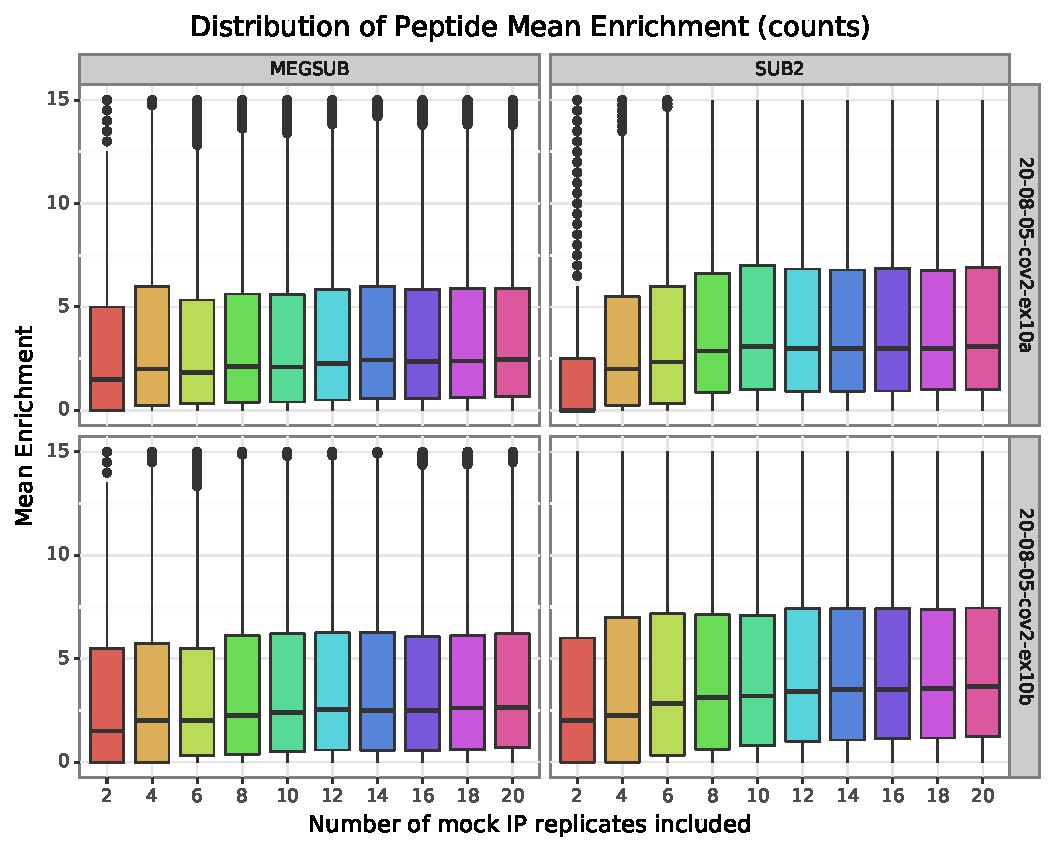
\includegraphics[width=85mm]{figures/42_mockip_abundance_variance/counts/mean_limit_y.pdf} &   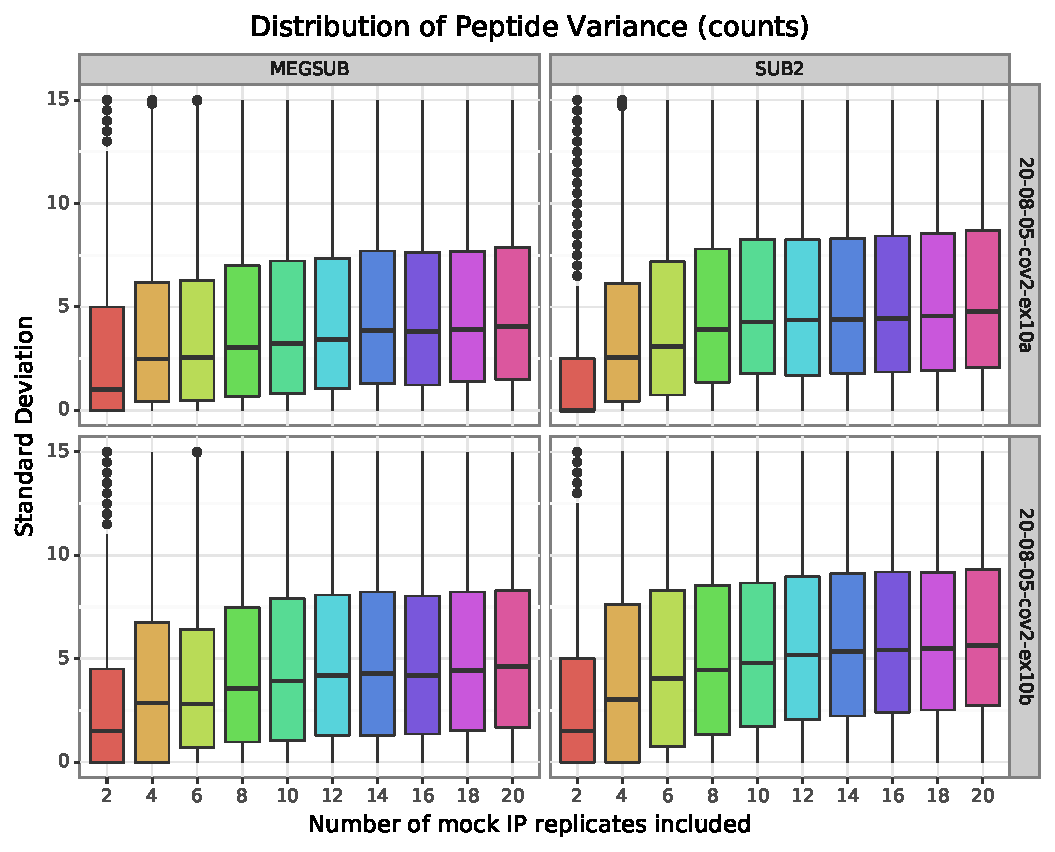
\includegraphics[width=85mm]{figures/42_mockip_abundance_variance/counts/std_limit_y.pdf} \\
%(a) first & (b) second \\[6pt]
% \includegraphics[width=85mm]{figures/42_mockip_abundance_variance/counts/mean.pdf} &   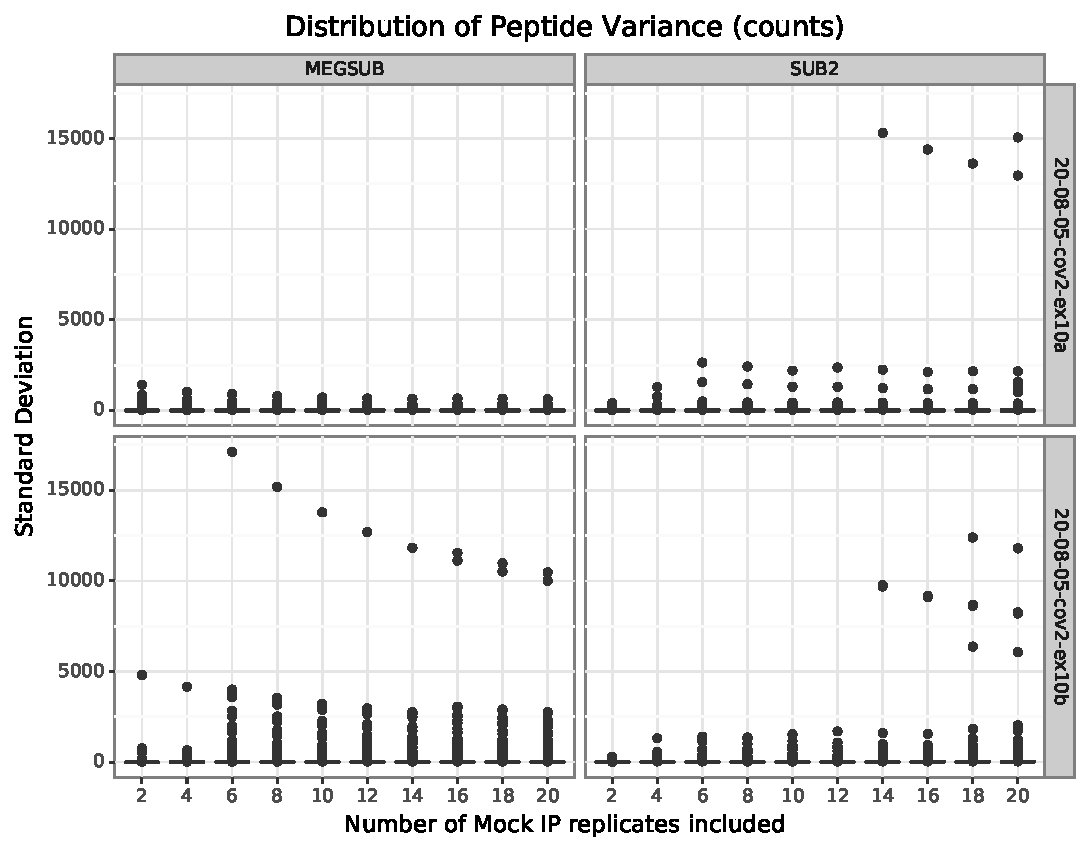
\includegraphics[width=85mm]{figures/42_mockip_abundance_variance/counts/std.pdf} \\
%(c) third & (d) fourth \\[6pt]
%\multicolumn{2}{c}{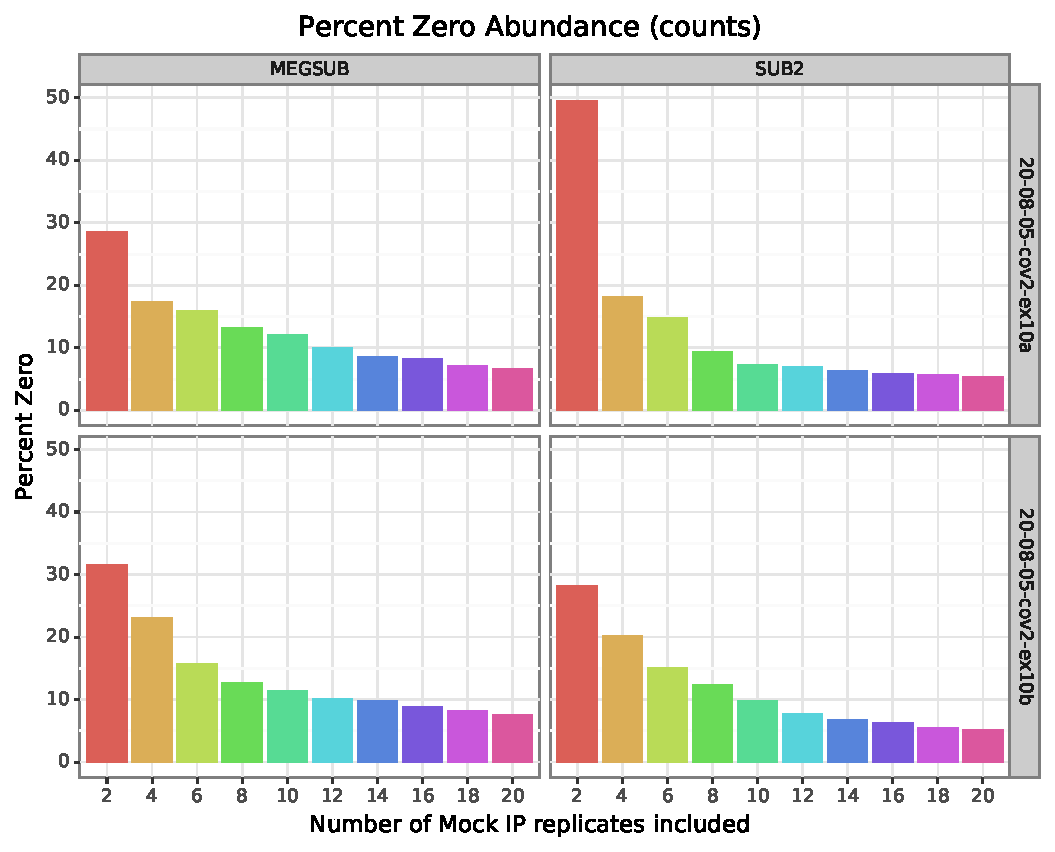
\includegraphics[width=105mm]{figures/42_mockip_abundance_variance/counts/per-zero.pdf} }\\
%\multicolumn{2}{c}{(e) fifth}
%\end{tabular}
%\caption{caption}
%\end{figure}
%
%\begin{figure}
%\centering
%\begin{tabular}{cc}
%  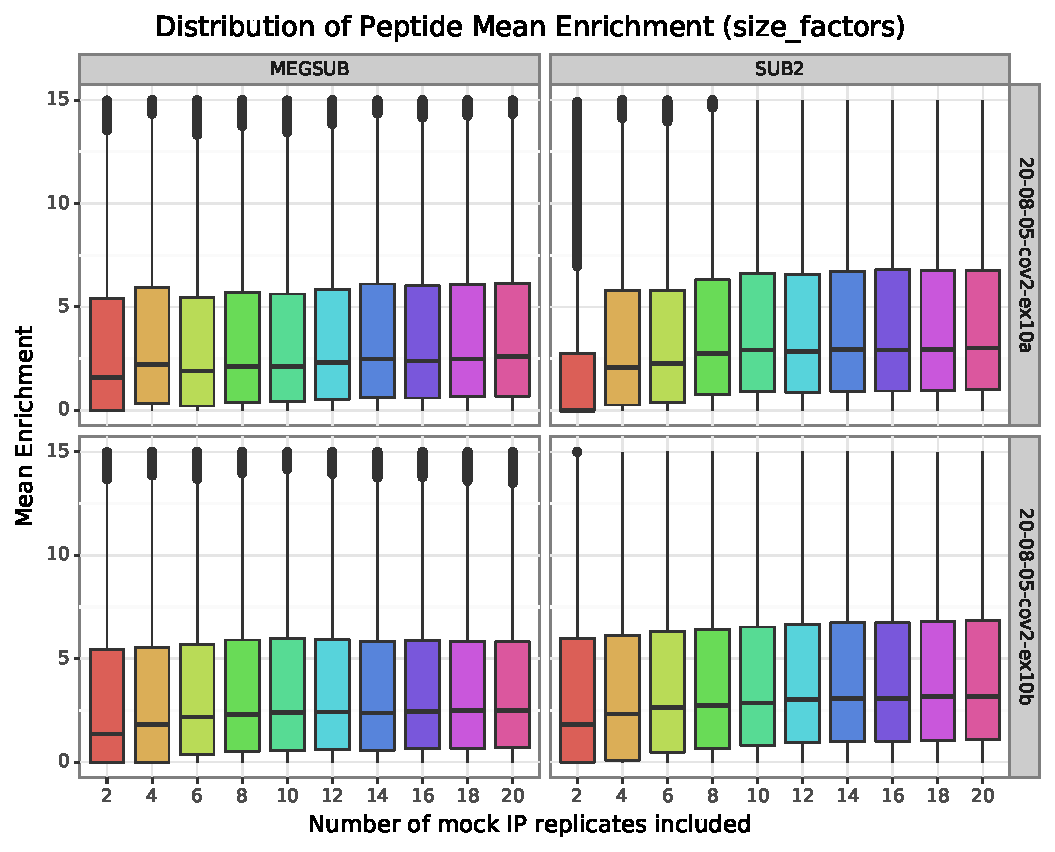
\includegraphics[width=85mm]{figures/42_mockip_abundance_variance/size_factors/mean_limit_y.pdf} &   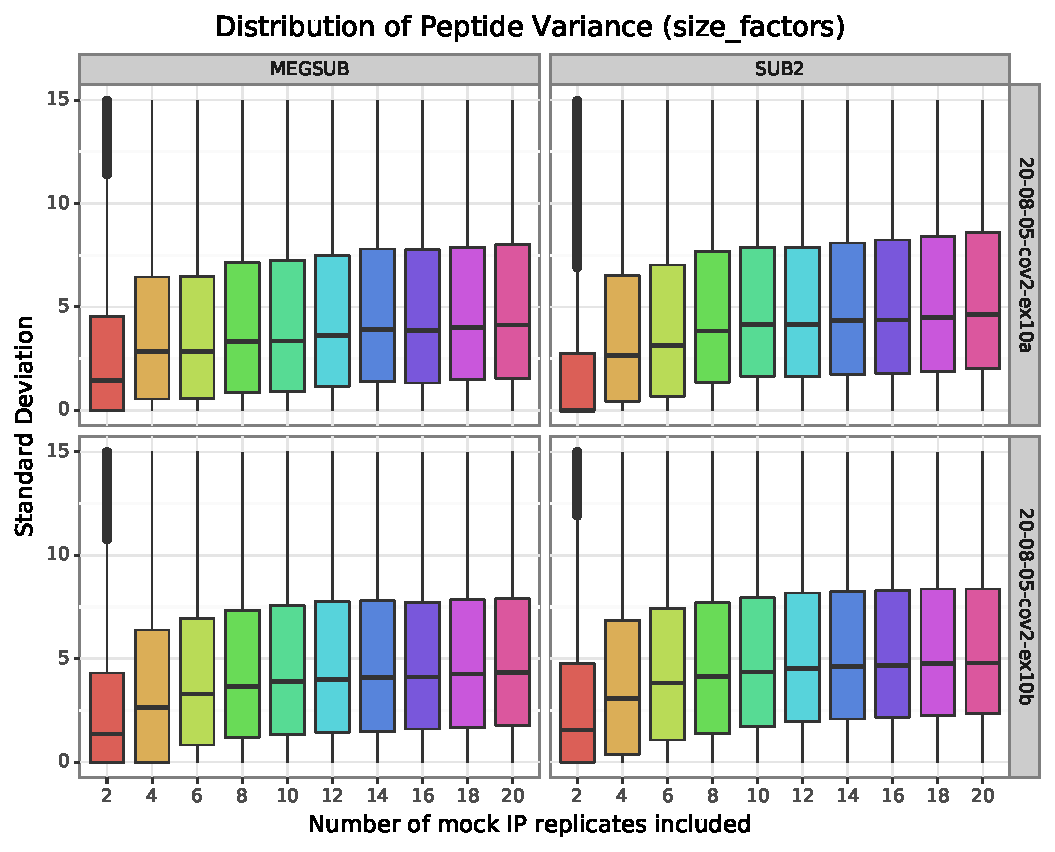
\includegraphics[width=85mm]{figures/42_mockip_abundance_variance/size_factors/std_limit_y.pdf} \\
%(a) first & (b) second \\[6pt]
% \includegraphics[width=85mm]{figures/42_mockip_abundance_variance/size_factors/mean.pdf} &   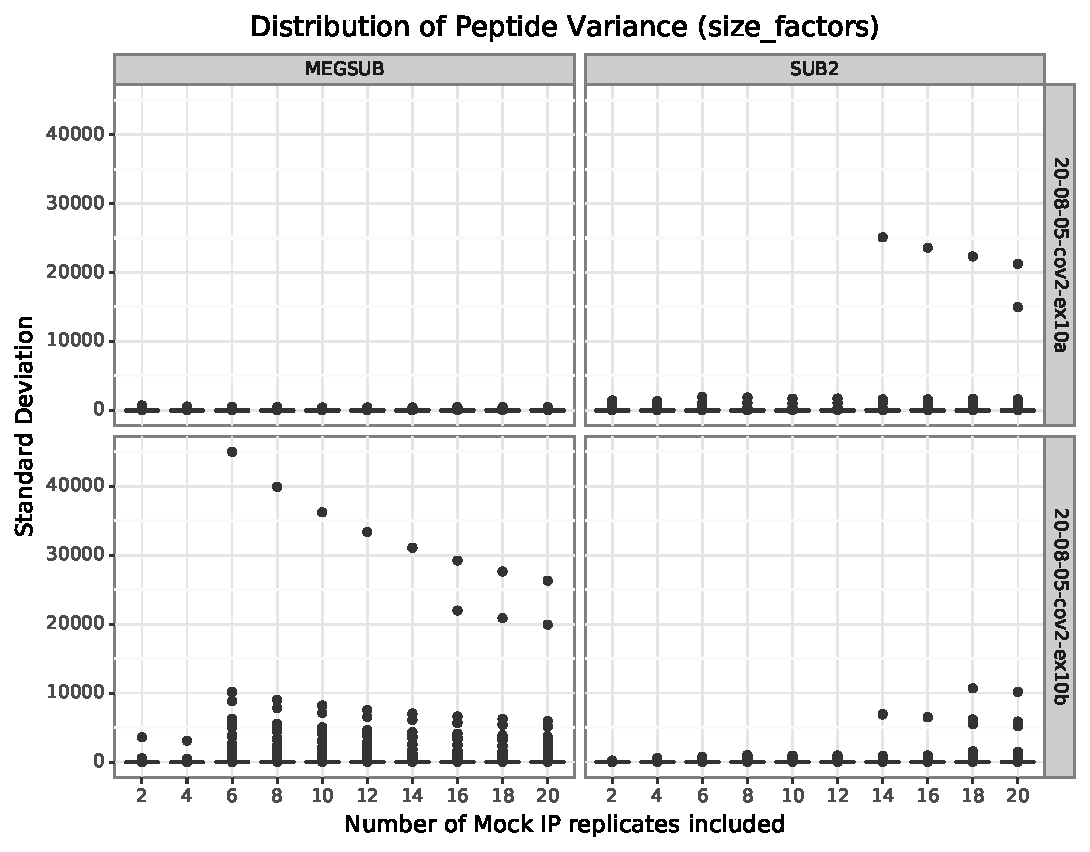
\includegraphics[width=85mm]{figures/42_mockip_abundance_variance/size_factors/std.pdf} \\
%(c) third & (d) fourth \\[6pt]
%\multicolumn{2}{c}{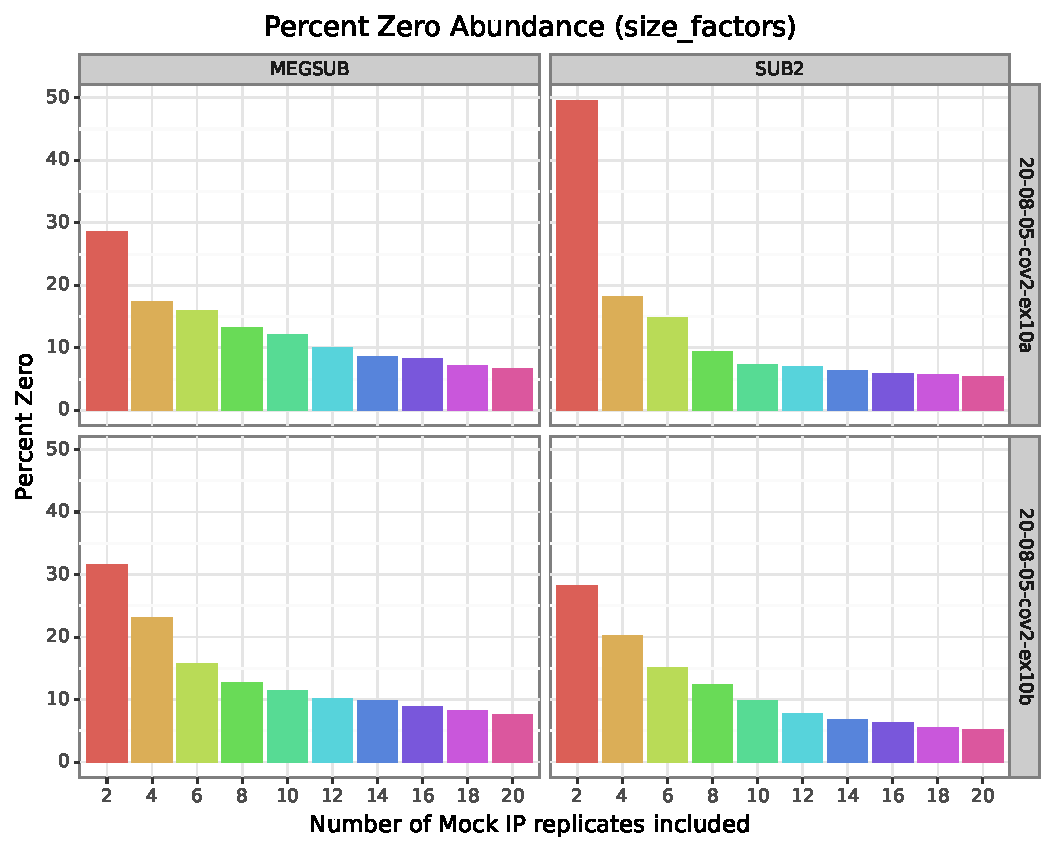
\includegraphics[width=105mm]{figures/42_mockip_abundance_variance/size_factors/per-zero.pdf} }\\
%\multicolumn{2}{c}{(e) fifth}
%\end{tabular}
%\caption{caption}
%\end{figure}

\subsection*{Deep Mutational Scanning}

\subsection*{Analysis and modeling}

\section*{Future Perspectives and Conclusions}




% \begin{figure}[h]
% \centering
% \includegraphics[width=0.35\textwidth]{figures/subsplit.pdf}
% \caption{\
% A subsplit structure.
% }%
% \label{fig:subsplit}
% \end{figure}


% \bibliographystyle{plain}
% \bibliography{main}

\bibliographystyle{plainnat}
\bibliography{main}

% \clearpage
% \section*{Supplementary Materials}
% \beginsupplement
% Supplementary text and figures here.


\end{document}
